% UQ Gemini theme - clean version with your content only
% Based on: https://github.com/alfurka/gemini-uq

\documentclass[final]{beamer}

% ====================
% Packages
% ====================

\usepackage[T1]{fontenc}
\usepackage{lmodern}
\usepackage[size=custom,width=100,height=75,scale=1.0]{beamerposter}
\usetheme{gemini}
\usecolortheme{uchicago}
\usepackage{graphicx}
\usepackage{booktabs}
\usepackage{tikz}
\usepackage{pgfplots}
\pgfplotsset{compat=1.17}
\usepackage[table]{xcolor}  % needed for rowcolors in your table

% ====================
% Lengths
% ====================

\newlength{\sepwidth}
\newlength{\colwidth}
\setlength{\sepwidth}{0.025\paperwidth}
\setlength{\colwidth}{0.3\paperwidth}

\newcommand{\separatorcolumn}{\begin{column}{\sepwidth}\end{column}}

% ====================
% Title, Author, Institute
% ====================

\title{The Impact of Prompt Engineering on Code Generation Accuracy and Hallucination Patterns in Language Models}

\author{Kadin Matotek \inst{1} \and Linh B. Ngo \inst{1}}

\institute[shortinst]{\inst{1} West Chester University, Department of Computer Science}

% ====================
% Footer
% ====================

\footercontent{
  Research conducted at WCU AIR Lab \hfill
  SICCS 2025 --- Poster Session \hfill
  \href{mailto:km998744@wcupa.edu}{km998744@wcupa.edu}
}

% ====================
% Logos (uncomment and adjust paths if you have logos)
% ====================

\logoright{\includegraphics[height=7cm]{figures/icon.png}}
\logoleft{\includegraphics[height=7cm]{figures/icon.png}}

% Optional: custom logo placement in header (kept from original template style)


% ====================
% Document
% ====================

\begin{document}

\begin{frame}[t]
\begin{columns}[t]
\separatorcolumn

% ==================== Column 1 ====================
\begin{column}{\colwidth}

\begin{block}{Introduction}
Large Language Models (LLMs) have demonstrated remarkable capabilities in code generation, yet their reliability remains a critical concern. This study investigates how different prompt engineering strategies affect model accuracy and hallucination patterns across coding tasks.

\textbf{Research Questions}
\begin{itemize}
  \item How do concise versus verbose instructions impact code generation accuracy?
  \item What types of errors and hallucinations emerge across different model sizes?
  \item How do reasoning strategies (Chain-of-Thought, Direct, Program-Aided) affect performance?
\end{itemize}
\end{block}

\begin{block}{Methodology}
We evaluated 5 Qwen model variants (0.5B to 14B parameters) on 3,230 programming problems using a systematic prompt engineering framework.

\textbf{Experimental Design}
\begin{itemize}
  \item \textbf{Base Instructions:} Concise vs. Verbose
  \item \textbf{Reasoning Strategies:} Chain-of-Thought, Direct, Program-Aided
  \item \textbf{Problem Decomposition:} None vs. Basic
  \item \textbf{Output Formats:} Code only, Explanation + Code, Code + Explanation
  \item \textbf{Total Configurations:} 36 prompt variants per model
  \item \textbf{Dataset:} 116,280 total test cases
\end{itemize}

\begin{figure}
  \centering
  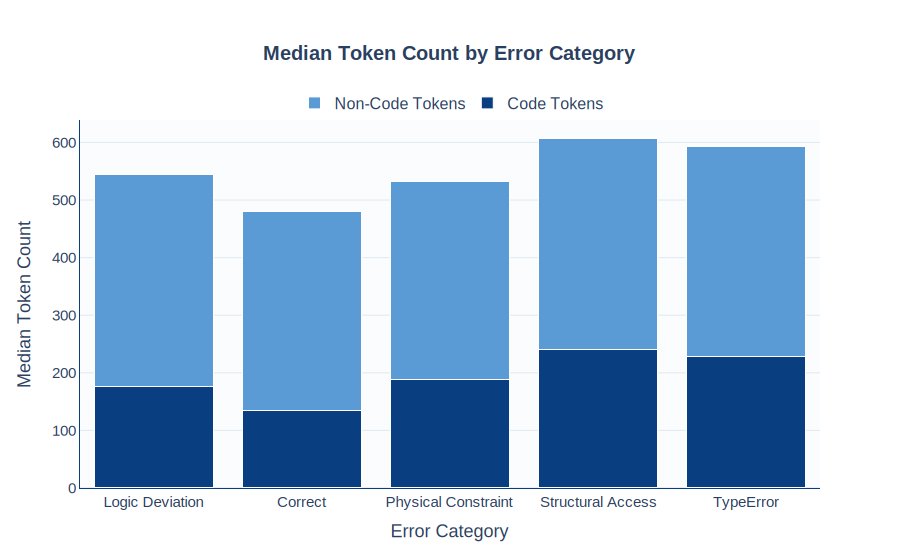
\includegraphics[width=0.95\linewidth]{figures/token_efficiency.png}
  \caption{Experimental framework showing prompt construction pipeline and evaluation methodology.}
\end{figure}
\end{block}

\begin{alertblock}{Key Finding: Conciseness Advantage}
Across all 18 prompt configuration comparisons, \textbf{concise instructions outperformed verbose ones in 94.4\%} of cases with an average improvement of +1.35\%.

This effect was most pronounced in smaller models, suggesting that verbose instructions may introduce noise that degrades performance.
\end{alertblock}

\end{column}
\separatorcolumn

% ==================== Column 2 ====================
\begin{column}{\colwidth}

\begin{block}{Results: Prompt Strategy Performance}

\textbf{Top Performing Configurations}

\begin{table}
\centering
\small
\rowcolors{2}{white!15!purple}{white}
\begin{tabular}{l l l l r}
\toprule
\textbf{Base} & \textbf{Reasoning} & \textbf{Decomp} & \textbf{Output} & \textbf{Acc \%} \\
\midrule
Concise & CoT      & None & Exp + Code & 32.07 \\
Concise & Direct   & None & Code only  & 31.95 \\
Concise & Direct   & None & Exp + Code & 31.83 \\
Concise & CoT      & None & Code only  & 31.67 \\
\midrule
Verbose & CoT      & None & Code only  & 30.71 \\
Verbose & Direct   & Basic & Code only & 30.19 \\
\bottomrule
\end{tabular}
\caption{Accuracy of top prompt configurations (n=3,230 per config).}
\end{table}

\textbf{Biggest Performance Gaps}
\begin{itemize}
  \item Direct reasoning, no decomposition, code-only output: \textbf{+2.88\%}
  \item Chain-of-Thought with explanation + code: \textbf{+2.26\%}
\end{itemize}

\end{block}

\begin{block}{Model Size Effects}
\begin{figure}
  \centering
  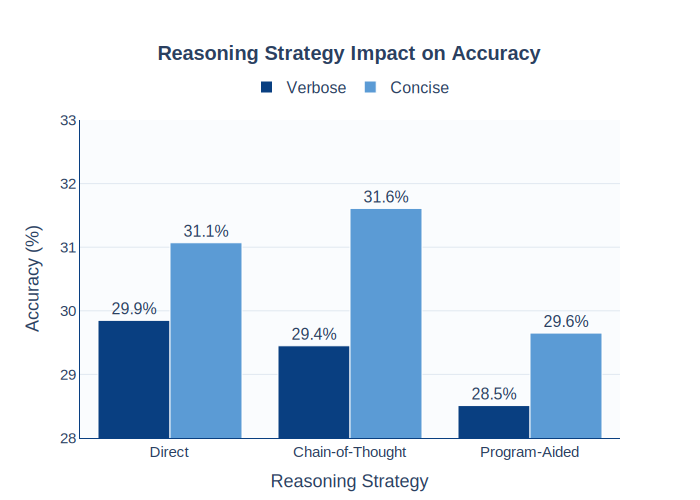
\includegraphics[width=0.95\linewidth]{figures/reasoning_strategy.png}
  \caption{Accuracy comparison showing concise prompts consistently outperform verbose across all model sizes. The advantage diminishes as models grow larger.}
\end{figure}

Smaller models showed greater sensitivity to prompt verbosity, with relative improvements from \textbf{+21.0\%} (0.5B) to \textbf{+0.4\%} (14B).
\end{block}

\end{column}
\separatorcolumn

% ==================== Column 3 ====================
\begin{column}{\colwidth}

\begin{block}{Error and Hallucination Analysis}
We categorized 28 distinct error types, revealing systematic failure patterns.

\textbf{Most Common Error Types}
\begin{itemize}
  \item \textbf{Logic Deviation} (41.6\%): Incorrect algorithmic approach
  \item \textbf{ValueError} (12.9\%): Invalid input handling
  \item \textbf{TypeError} (2.9\%): Type mismatches
  \item \textbf{IndexError} (3.1\%): Array boundary violations
  \item \textbf{NameError} (2.8\%): Undefined variables
\end{itemize}

\begin{figure}
  \centering
  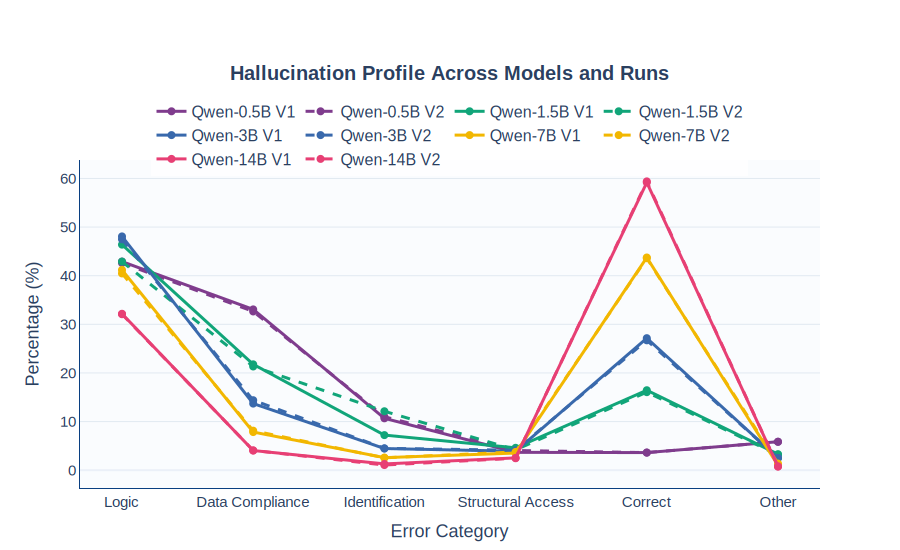
\includegraphics[width=0.95\linewidth]{figures/hallucination_stability.png}
  \caption{Distribution of error types across model sizes. Logic deviations dominate but decrease with model capacity.}
\end{figure}
\end{block}

\begin{block}{Token Usage Patterns}
\begin{figure}
  \centering
  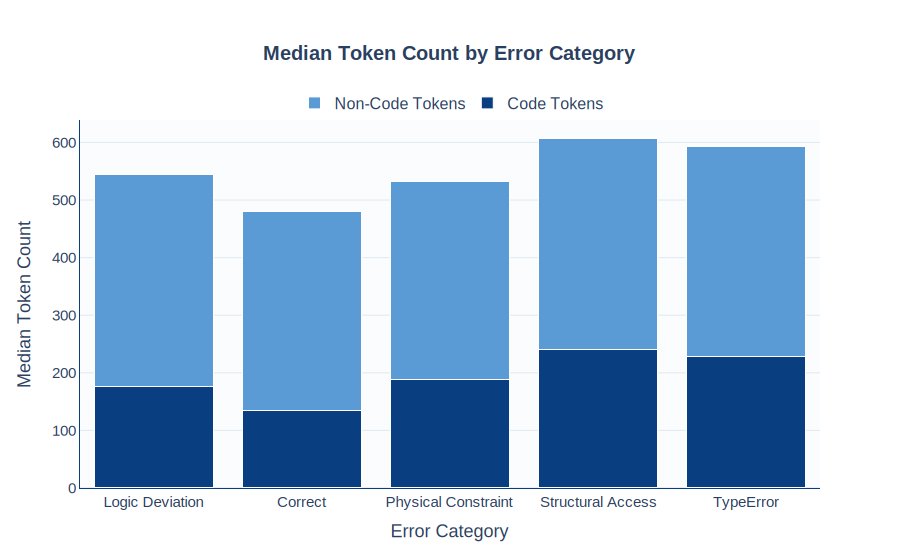
\includegraphics[width=0.95\linewidth]{figures/token_efficiency.png}
  \caption{Median token counts for correct vs. incorrect responses.}
\end{figure}

Correct solutions used 343–501 median tokens depending on model size. Logic deviation errors showed similar token usage, indicating verbosity alone is not predictive of correctness.
\end{block}

\begin{block}{Conclusions and Future Work}

\textbf{Key Takeaways}
\begin{itemize}
  \item Concise prompts consistently outperform verbose alternatives
  \item Smaller models are more sensitive to prompt engineering
  \item Logic deviations are the dominant failure mode
  \item Reasoning strategy and output format significantly affect accuracy
\end{itemize}

\textbf{Future Directions}
\begin{itemize}
  \item Investigate optimal prompt length thresholds
  \item Develop targeted mitigation for logic deviations
  \item Extend to other model families and domains
  \item Explore automated prompt optimization
\end{itemize}

\end{block}

\begin{block}{References}
\nocite{*}
\small\bibliographystyle{plain}\bibliography{poster}
\end{block}

\end{column}
\separatorcolumn

\end{columns}
\end{frame}

\end{document}